% !TeX encoding = UTF-8
% !TeX spellcheck = hu_HU

\chapter{Technológiai áttekintés}
\label{chap:technologies}

\section{Szervergépek}
\label{sect:servers}
A szerverek esetében jelentkező, egyénitől nagyban különböző felhasználási körülmények a szerverszámítógépek esetén hardveres szempontból is más felépítést igényelnek. A magas rendelkezésre-állás (\acrlong{ha}, \acrshort{ha}) és a modularitás, valamint az ezzel járó könnyű javítások támogatása érdekében az ilyen célra kialakított számítógépek főbb komponensei redundánsak, azaz egy-egy ilyen komponens kiesése nem jelent szolgáltatáskiesést. A meghibásodást a rendszer egyértelműen jelzi magán a gépházon is (általában hibajelző LED-ek segítségével), valamint a menedzsment portjain is. A legtöbb ilyen gép ugyanis rendelkezik egy beágyazott rendszerrel, ami lehetővé teszi a távoli kezelésüket egy webes felületen és SSH-n keresztül még akkor is, ha a szervergép ki van kapcsolva. Ezek lehetőséget biztosítanak a gép legfontosabb mérőszámainak követésére, virtuális kijelző csatlakoztatására, telepítőfájlok felcsatolására, valamint a gép ki- és bekapcsolására.

\begin{figure}[!ht]
	\centering
	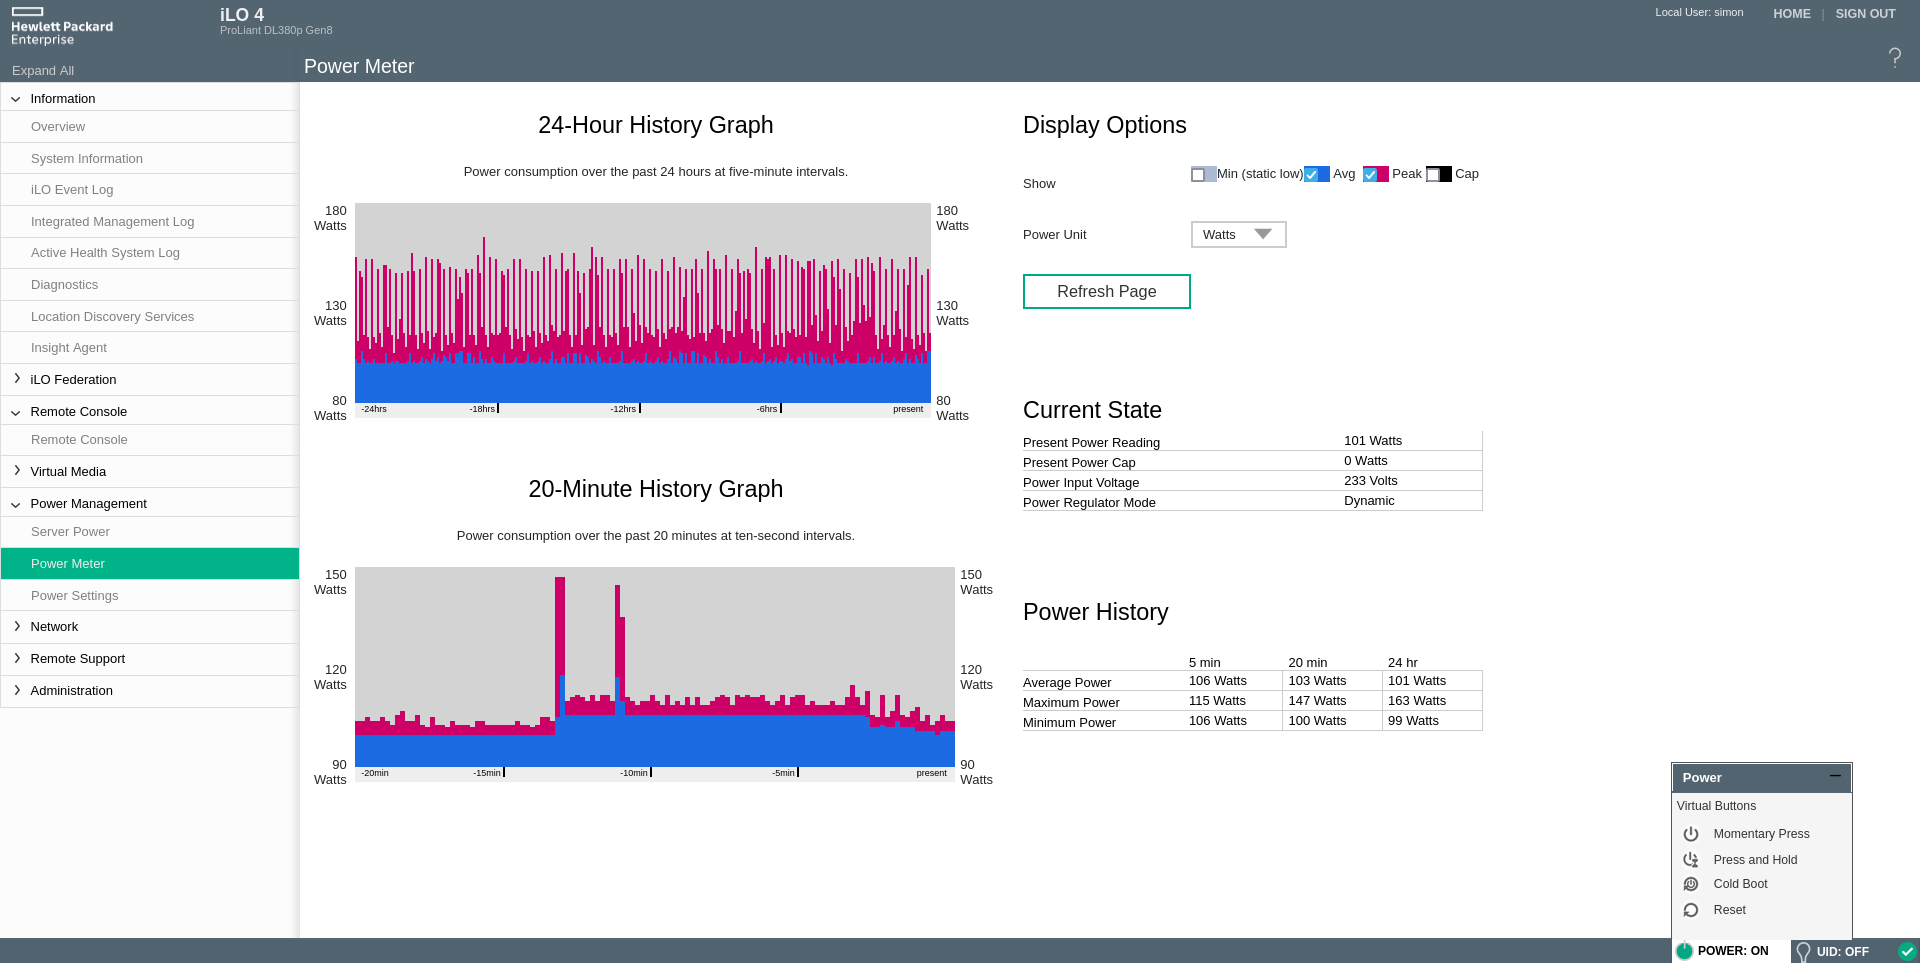
\includegraphics[width=150mm, keepaspectratio]{figures/ilo-power1.png}
	\caption{Szervergép fogyasztásának grafikonja egy HPE számítógép távoli menedzsment felületén. Vegyük észre a jobb alsó sarokban megjelenő menüt, amivel lehetőségünk van a gép kikapcsolására és újraindítására is.}
	\label{fig:ilopowerchart}
\end{figure}

A fent ismertetett üzemeltetést, karbantartást könnyítő felépítés mellett általában elmondható, hogy az ilyen gépek jelentős része virtualizációra van tervezve -- persze ezektől különböző felhasználási módok is jelentkeznek (például fájlszerverek tervezése során a teljesítmény helyett a minél nagyobb tárkapacitásra és adatátvitelre helyezték a hangsúlyt). A dolgozat szempontjából viszont a nagyvállalati környezetben domináló virtualizációs felhasználási terület lesz a lényegesebb, így a továbbiakban az ilyen számítógépekre fogok koncentrálni.

A virtualizációs hosztgépek jellemzője, hogy számos processzorral rendelkeznek, valamint felhasználói szemmel szokatlanul nagy memóriaterülettel bírnak. Ki fog derülni azonban, hogy 12-24 processzormag és akár több száz gigabyte RAM is szűkös erőforrássá válhat egy virtuális gépeket futtató számítógép esetében, hiszen gyakorlatilag itt egyetlen szervernek kell elbírnia akár több tíz számítógép terhelésével is. Ezek mellett általában több (8-24) háttértár-foglalattal is rendelkeznek, melyekhez hardveres RAID-támogatást is adnak.
% TODO: kép a gépről

\section{Virtualizáció}
\subsection{Áttekintés}
A virtualizáció egy olyan technológia, amely lehetővé teszi, hogy egy fizikai számítógépen (az úgynevezett virtuális host-on) több, akár a hosztgép rendszerétől eltérő operációs rendszert futtassunk. Ehhez szükség van egy \gls{hypervisor}-ra, ami az operációs rendszer legfőbb virtualizációt támogató komponense~\cite{Sles15virt}. Ez a szoftver közvetlenül a szerver hardverén fut, és ez biztosítja a virtuális gépek számára szükséges hardveres erőforrásokat virtualizált hardverinterfészeken keresztül. Szintén a \gls{hypervisor} felelős az erőforrások kezeléséért, tehát ennek a komponensnek kell biztosítania a virtuális gép számára beállított mennyiségű memória, processzor és háttértár rendelkezésre állását is. Ezek a beállítások a legtöbb modern \gls{hypervisor} esetében elvégezhetőek grafikus felületen is, erre ad példát \aref{fig:vboxsettings} ábra.

Napjainkban a legelterjedtebb hypervisorok közé tartozik a VMware ESXi, a XEN és a KVM, melyek részletesebb bemutatását \aref{sect:hypervisor-comparision} alfejezet tartalmazza.

\begin{figure}[!ht]
	\centering
	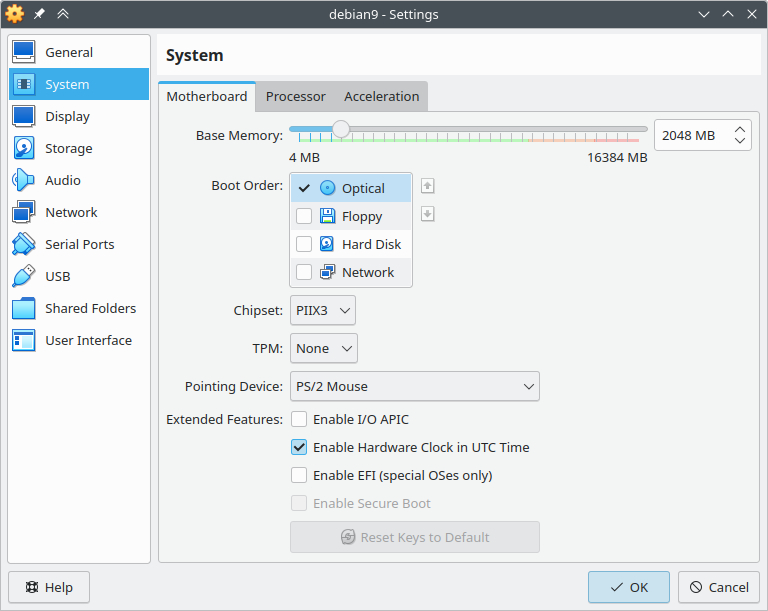
\includegraphics[width=120mm, keepaspectratio]{figures/virtualbox-vm-settings.png}
	\caption{Virtuális gép beállításainak részlete a VirtualBox virtualizációs szoftverben.}
	\label{fig:vboxsettings}
\end{figure}


A virtualizáció számos előnnyel járhat az infrastruktúra és a kiszolgálni kívánt alkalmazások szempontjából. Az egyik legnagyobb ilyen előny például, hogy a virtuális gépek egymástól izoláltan futnak, azaz nincs közvetlen kapcsolat közöttük, ami biztonsági és kezelési, tesztelési szempontból (pl. egy adott csomag vagy szoftver kipróbálásához készíthetünk egy teszt virtuális gépet, amit egyszerűen törölhetünk a teszt végeztével; a telepített program eltávolítása hagyományos környezetben futtatva sokkal körülményesebb lenne) is kedvező lehet. Hasonlóan előnyökkel jár, hogy a legtöbb modern \gls{hypervisor} lehetőséget biztosít bizonyos erőforrások úgynevezett \gls{hotswap}-pelésére. Ez azt jelenti, hogy egyes komponenseket (pl. memória) úgy is bővíthetünk, hogy a rendszert nem szükséges ehhez leállítanunk.

\subsection{Paravirtualizáció és teljes virtualizáció}

\subsection{Virtualizációs lehetőségek összehasonlítása} \label{sect:hypervisor-comparision}



\section{Virtualizáció}
A fent említett megnövekedett forgalom kiszolgálását hatékonyan lehet kezelni úgy, hogy olyan fizikai számítógépet helyezünk üzembe, mely  több, egymástól független operációs rendszer futtatására is alkalmas. Ilyenkor ezeket a fizikai gépen futó rendszereket virtuális gépeknek (\acrlong{vm}, \acrshort{vm}) nevezzük. Egy virtuális gép elkülönített erőforrásokat kap a fizikai géptől, hozzáférhet például bizonyos mennyiségű processzormaghoz, memóriához, illetve külön háttértár-partíciói is lehetnek. A virtualizált hardverek és operációs rendszerek a legtöbb esetben a külvilág felé nem különböztethetőek meg a fizikai számítógépektől, és ezzel a megoldással jelentősen csökkenthető a rendszerek és a hozzájuk szükséges informatikai infrastruktúra üzemeltetésének költsége.

A virtualizáció nagy ereje abban rejlik, hogy bizonyos hardverek virtualizációjával egységnyi teljesítményt olcsóbban kaphatunk meg, mintha külön fizikai gépeket helyeznénk üzembe, illetve nagyobb rugalmasságot kapunk a kezelésükben, üzemeltetésükben. Képzeljük el, hogy megveszünk egy számítógépet, amin szeretnénk futtatni egy számunkra fontos alkalmazást, mondjuk a honlapunkat. Ilyenkor az ezen a gépen futó operációs rendszer teljes mértékben megszabhatja, hogy milyen erőforrásokból mennyit használ. Ha egy másik szolgáltatást -- például levelezőszervert -- szeretnénk emellett futtatni, akkor limitáltabbak a lehetőségeink, hiszen a korábban telepített webszerver már foglal bizonyos erőforrásokat, illetve a program függőségeit és konfigurációs fájljait is telepítettük már, ami esetleg negatívan hat a levelezőszerverünk működésére. Ha mindezt virtualizált környezetben tesszük meg, akkor a topológia megváltozik: a két alkalmazás teljesen elkülönítetten, egymás zavarása nélkül, különböző virtuális gépekben futhatnak, míg magán a fizikai gépen egy úgynevezett hypervisor látja el az erőforrások ütemezésének és kiosztásának (pl. processzoridő, memória) feladatát.
% TODO: virt-manager screenshot, esetleg virsh xml screenshot

\subsection{Népszerű virtualizációs technológiák}
Mivel a virtualizáció napjainkban nagyon elterjedt technológia, számos olyan megoldás született, mely egyszerűsíti a virtuális gépek üzemeltetését. Ezek közül nagy ismertségnek örvend az Oracle VirtualBox és a VMware Player, azonban ezek a megoldások nem skálázódnak annyira jól, mint a továbbiakban tárgyalt társaik, melyek sokkal megfelelőbbek nagyvállalati szerverkörnyezetben való alkalmazásra. Ezek a megoldások lehetőséget biztosítanak a virtuális gépek távoli elérésre, kezelésére, egyszerűbb telepítésükre, valamint szükség esetén elosztott működésükre.

Ilyen nagyvállalati környezetben is kedvelt megoldás például a VMware ESXi, amely egy igen modern hypervisor számos kényelmi funkcióval ellátva (lehetőség van például a rendszer webes felületről való kezelésére és virtuális gépek sablonból való gyors (nagyságrendileg 5-10 perc) telepítésére).
Egy másik kedvelt megoldás az ESXi-vel ellentétben teljesen ingyenesen, GPLv2-es licenc alatt elérhető XEN hypervisor, mely ugyan kevesebb kényelmi funkciót tartalmaz, de szintén népszerűségnek örvend széleskörű támogatása, kedvező teljesítménye és szabad szoftver voltából eredő ingyenessége miatt. A XEN a 2014 márciusában kiadott 4.4-es verzió óta stabilan működik együtt a libvirt virtualizációs \acrshort{api}-val, amely nagyban megkönnyíti a hypervisorral való kommunikációt a virtuális gépek konfigurálása során~\cite{Xen44ReleaseNotes}.

A XEN-hez hasonlóan szabad szoftver licenccel érhető el a \acrfull{kvm} is, mely a XEN-nél modernebb megoldásnak tekinthető, és manapság széles körben használják a Linux kernelbe való integráltságának és stabilitásának köszönhetően. Bár maga a \acrshort{kvm} nem tartalmaz ilyet, de számos interfész elérhető az ezen keresztül futtatott virtuális gépek kezelésére (például virt-manager), valamint akadnak olyan megoldások is, melyek a \acrshort{kvm}-re alapozva nyújtanak szélesebb körű virtualizációs megoldást, ilyen lehet\footnote{A konfigurációtól függően akár többfajta virtualizációs környezet is beállítható, de a \acrshort{kvm} az egyik legjobban támogatott.} például a Proxmox és a Cockpit.


\subsection{Virtuális gépek használatának néhány előnye}
A virtualizáció számos előnnyel bír a szerverinfrastruktúra karbantartása, könnyű kezelhetősége szempontjából, ebből néhány fontosabbat szeretnék kiemelni.

\subsubsection{Erőforrások testreszabása}
Amikor több tíz vagy több száz szerver üzemeltetéséről van szó, akkor hatványozottan számításba kell vennünk az egyes gépekre jutó költségeket. Virtuális gépek esetén ez azért kedvezőbb egy fizikai gépnél, mert ugyan a nagyvállalati környezetbe szánt szervergépek jelentősen drágábbak a személyes felhasználásra tervezett társaiknál, de akár több tíz virtuális gép egyidejű futtatását is lehetővé teszik. Ezáltal az egy fizikai gépre eső, asztali gépeknél megszokott áramfogyasztáshoz képest jóval nagyobb energiafelvétel sokkal kedvezőbb arányt mutat, ha számításba vesszük a futtatott virtuális kiszolgálók számát is.

Mindezek mellett a nagyvállalati felhasználáshoz tervezett számítógépek jóval hibatűrőbbek, hiszen a főbb komponensek redundánsan lettek kialakítva: ezekből az ilyen szerverekben legalább kettő van, és a rendszer automatikusan képes detektálni a hardveres hibákat, és ezek figyelembe vételével tovább működni. További előny lehet még hardveres hibák esetén, hogy ezek a számítógépek széles körben támogatják az úgynevezett \textit{hot swappingot}, amely azt jelenti, hogy bizonyos hardverelemek (általában például háttértárak és memóriamodulok) a számítógép bekapcsolt állapotában, annak működése közben is szolgáltatás nélkül cserélhetőek.

Előnyös lehet továbbá, hogy a virtuális gépek erőforrásai szabadon módosíthatók, így akár két újraindítás között is változtathatjuk a rendelkezésre álló memória mennyiségét vagy épp a processzormagok számát. Sőt, egyes hypervisorok és operációs rendszerek ezen erőforrások futásidejű megváltoztatását is támogatják bizonyos korlátozások mellett, így gyakorlatilag a fontosabb virtualizált erőforrások is hot swappelhetőnek tekinthetőek.

\subsubsection{Snapshotok}
Egy másik kedvező lehetőség virtuális gépek használata esetén az, hogy úgynevezett snapshotokat készíthetünk róluk. Ezek a snapshotok a gépet egy adott pillanatbeli állapotban reprezentálják, és később ezeket az állapotokat visszaállíthatjuk, ha szükségünk lesz rá. Egyes megoldások a memóriakép mentését is támogatják, így akár egy futó gép is könnyen visszaállítható. A snapshotok készítése hasznos lehet például rendszerfrissítések esetén, így ha valamiféle hiba lép fel a frissítés során, vagy egy adott szoftver nem megfelelően működik azt követően, akkor a frissítés előtt készített snapshotra visszaállva újra teljes értékűen üzemelhet a szerver, amíg a frissítés során fellépő hibát elhárítjuk.

\subsubsection{Migráció}
Részben az előző ponthoz kapcsolódik a virtuális gépek migrációja. Ez a funkció azt jelenti, hogy egy adott fizikai gépről, mely virtuális gépeket futtat (virtual host), készíthetünk egy snapshotot, amit áthelyezhetünk egy másik virtual hostra, és a virtuális gép ezen futhat tovább egyéb újrakonfigurálás nélkül.
Lehetőség van azonban a háttértárak tartalmát elhagyva is átmozgatni egy VM-et egy másik hosztra. Ehhez bevett szokás leírófájlok használata, mely egy virtuális gép konfigurációját tartalmazza. A leírófájlt egy másik hosztgépre áthelyezve ott újra elindíthatjuk a definiált virtuális gépet. Ilyenkor szükség lehet a VM háttértárainak inicializálására, de ettől eltekintve a konfiguráció szabadon hordozható virtual host-ok között. Ilyen migrációra egyes megoldások fejlettebb támogatást is adnak, így akár valós időben, az aktuális terheltség figyelembe vétele mellett automatikusan is áthelyezhetőek virtuális gépek a megadott fizikai hosztok között.
% TODO: listing egy példa virsh xml-lel

\subsection{Teljes virtualizáció és paravirtualizáció összehasonlítása}
\subsection{Konténerizáció}

\section{Logikai kötetkezelés}
\subsection{Snapshotok, mentések készítése}




[TODO: vmware a könnyű kezelhetőség és jó támogatás miatt magasan az élen áll; XEN, KVM]


\section{RAID}
Nagyvállalati környezetben nem hagyhatjuk ki a RAID-megoldásokat (a népszerű RAID 1 és RAID 6 megoldásokat \az{\ref{fig:raid} ábra} szemlélteti), ha adatok biztonsági mentéséről beszélünk. Ezek arra adnak lehetőséget, hogy az adatokat több háttértáron (pl. merevlemez vagy SSD) tároljuk úgy, hogy egy esetleges diszk hiba ne okozzon fennakadást a működésben. Fontos tisztában lenni azonban azzal, hogy a RAID-megoldások nem védenek bizonyos veszélyek ellen (például zsarolóvírusok, fájlok korruptálódása), hiszen az adatok duplikálása valós időben történik, így egy esetleges támadás során a RAID pool-ba bevont összes diszken megváltoznak az adatok, így nem alkalmas a támadás utáni visszaállításra. Emiatt egy RAID pool a \textit{3-2-1} mentési stratégiát alkalmazva csak egyetlen eszköznek tekinthető, hiába több lemezt használunk a mentés során. RAID-elést tehát csak hardveres hibák ellen érdemes használnunk, rosszindulatú támadás esetén ezek nem nyújtanak védelmet az adataink számára.

% TODO: RAID ábra, hivatkozások
\begin{figure}[!ht]
	%	\centering
	%	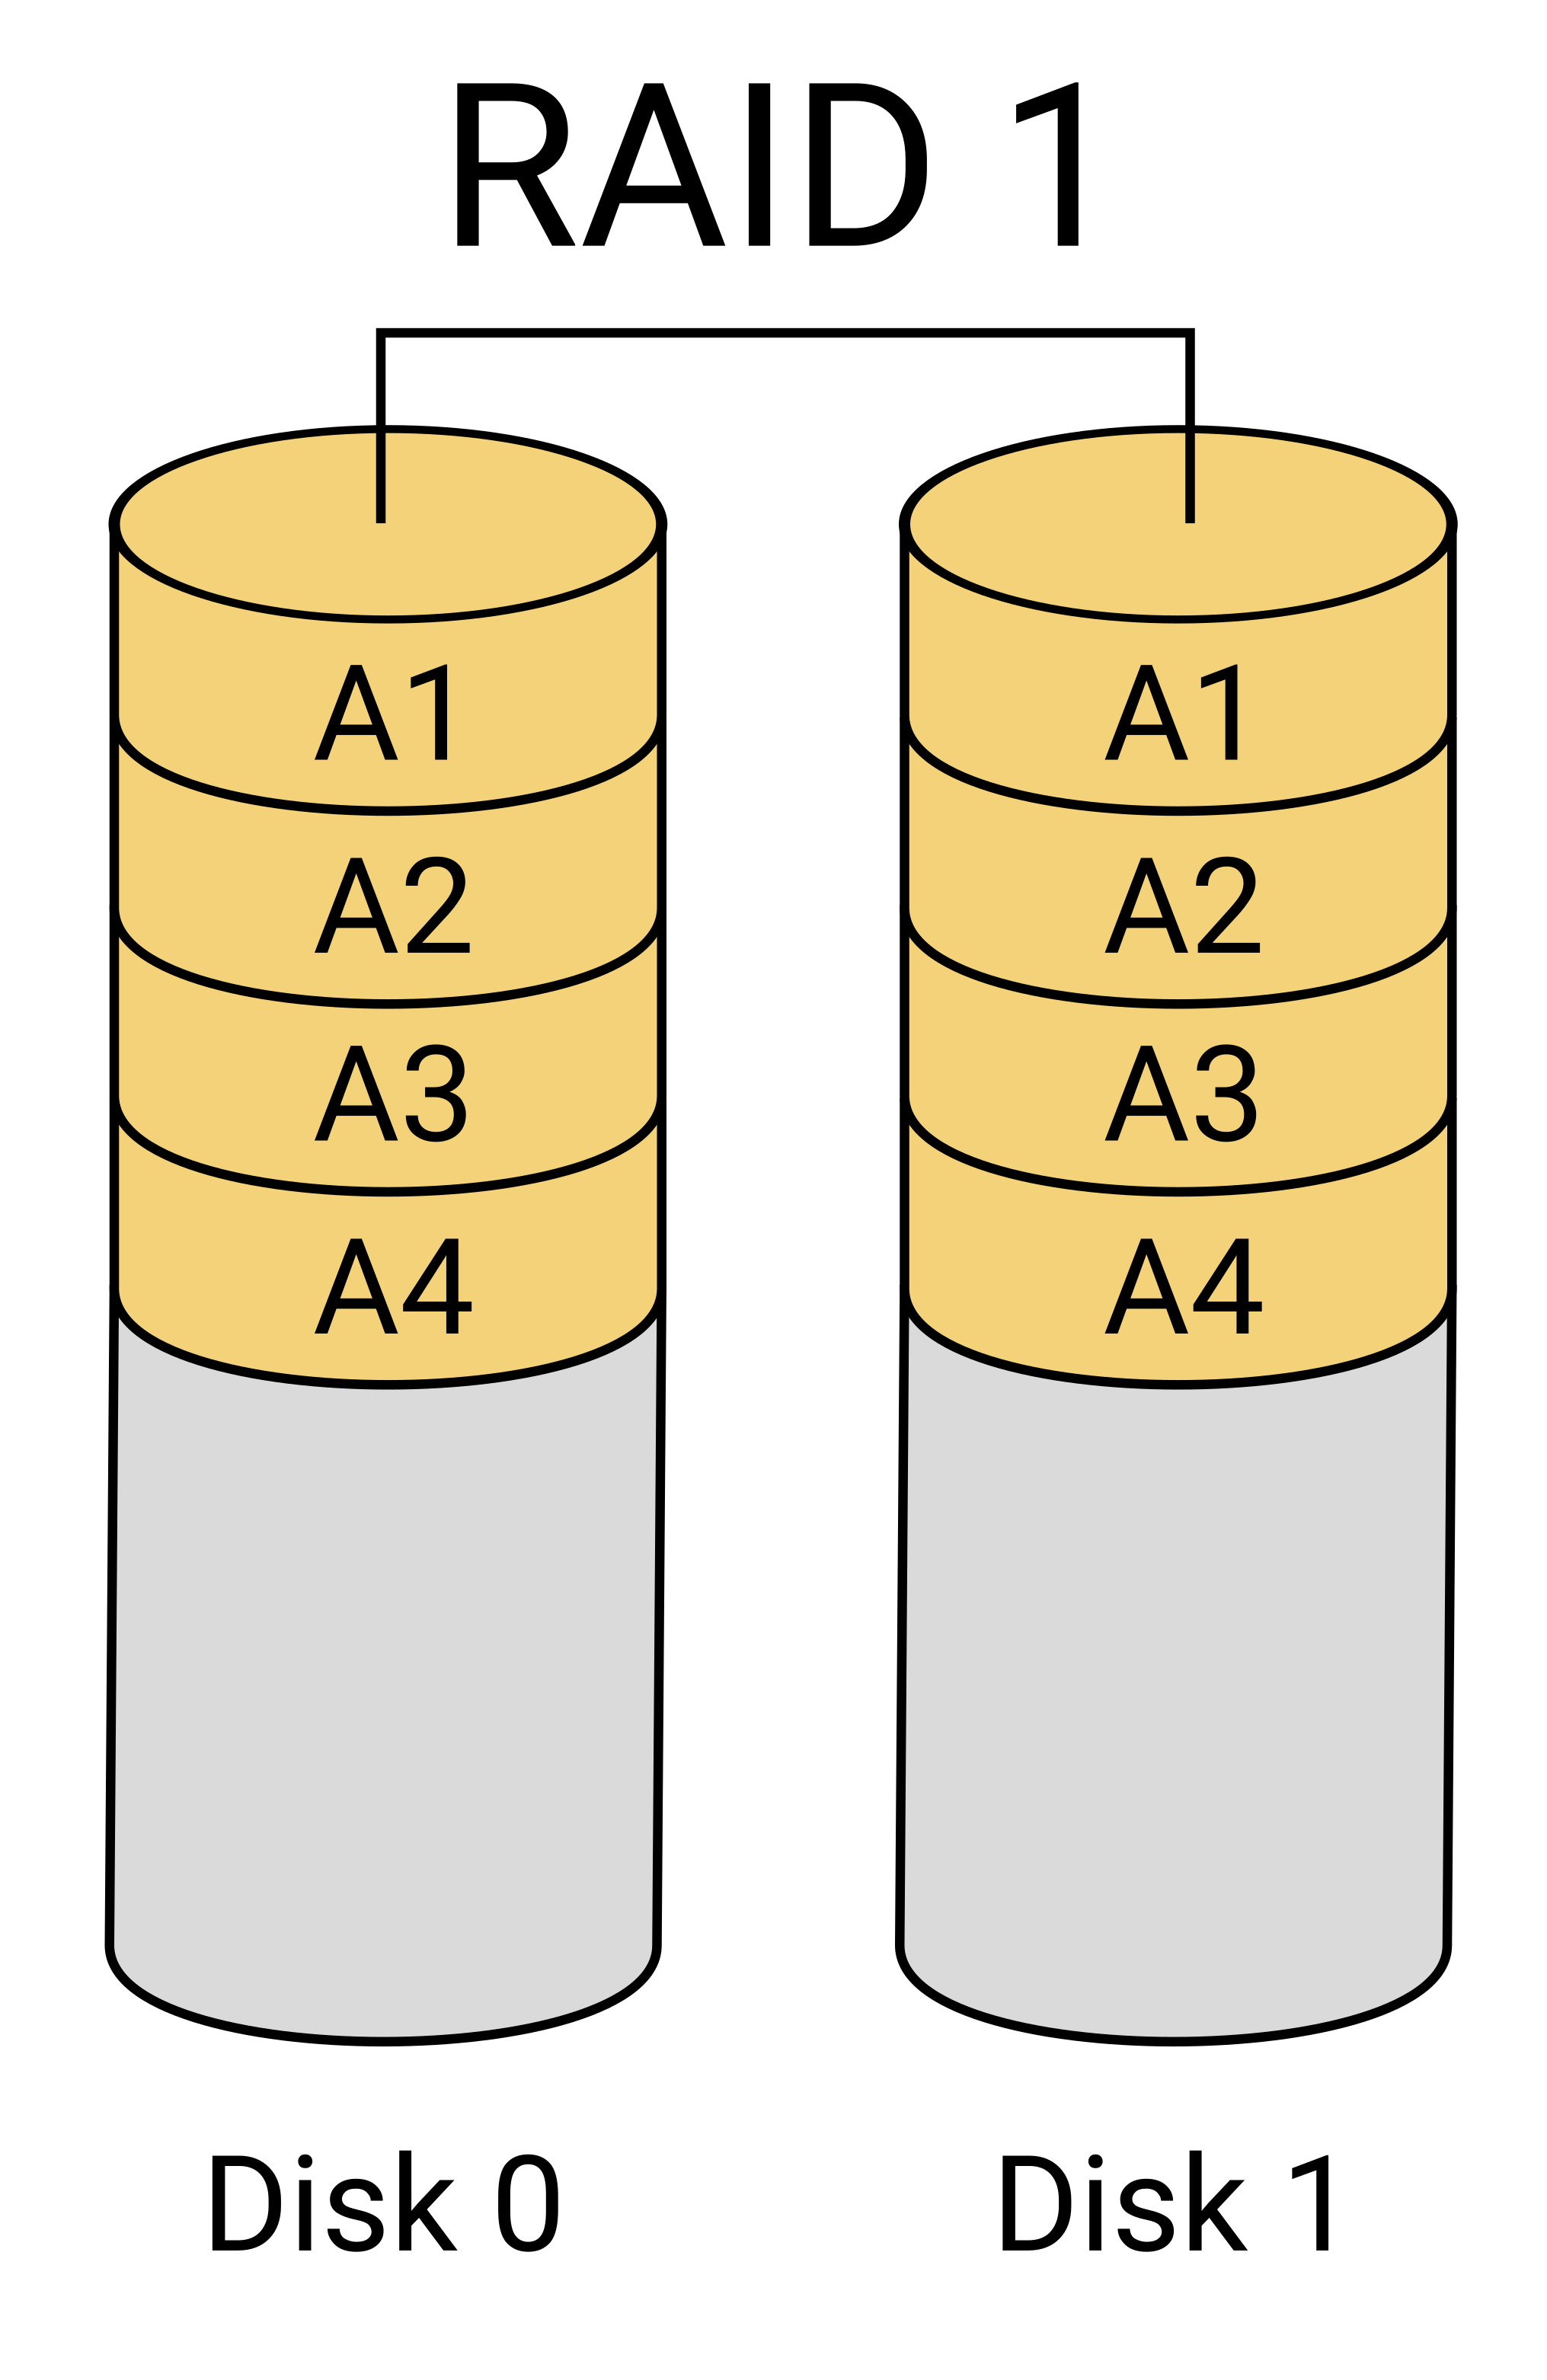
\includegraphics[height=70mm, keepaspectratio]{figures/raid1.pdf}
	
	\centering
	\begin{subfigure}{0.3\textwidth}
		\centering
		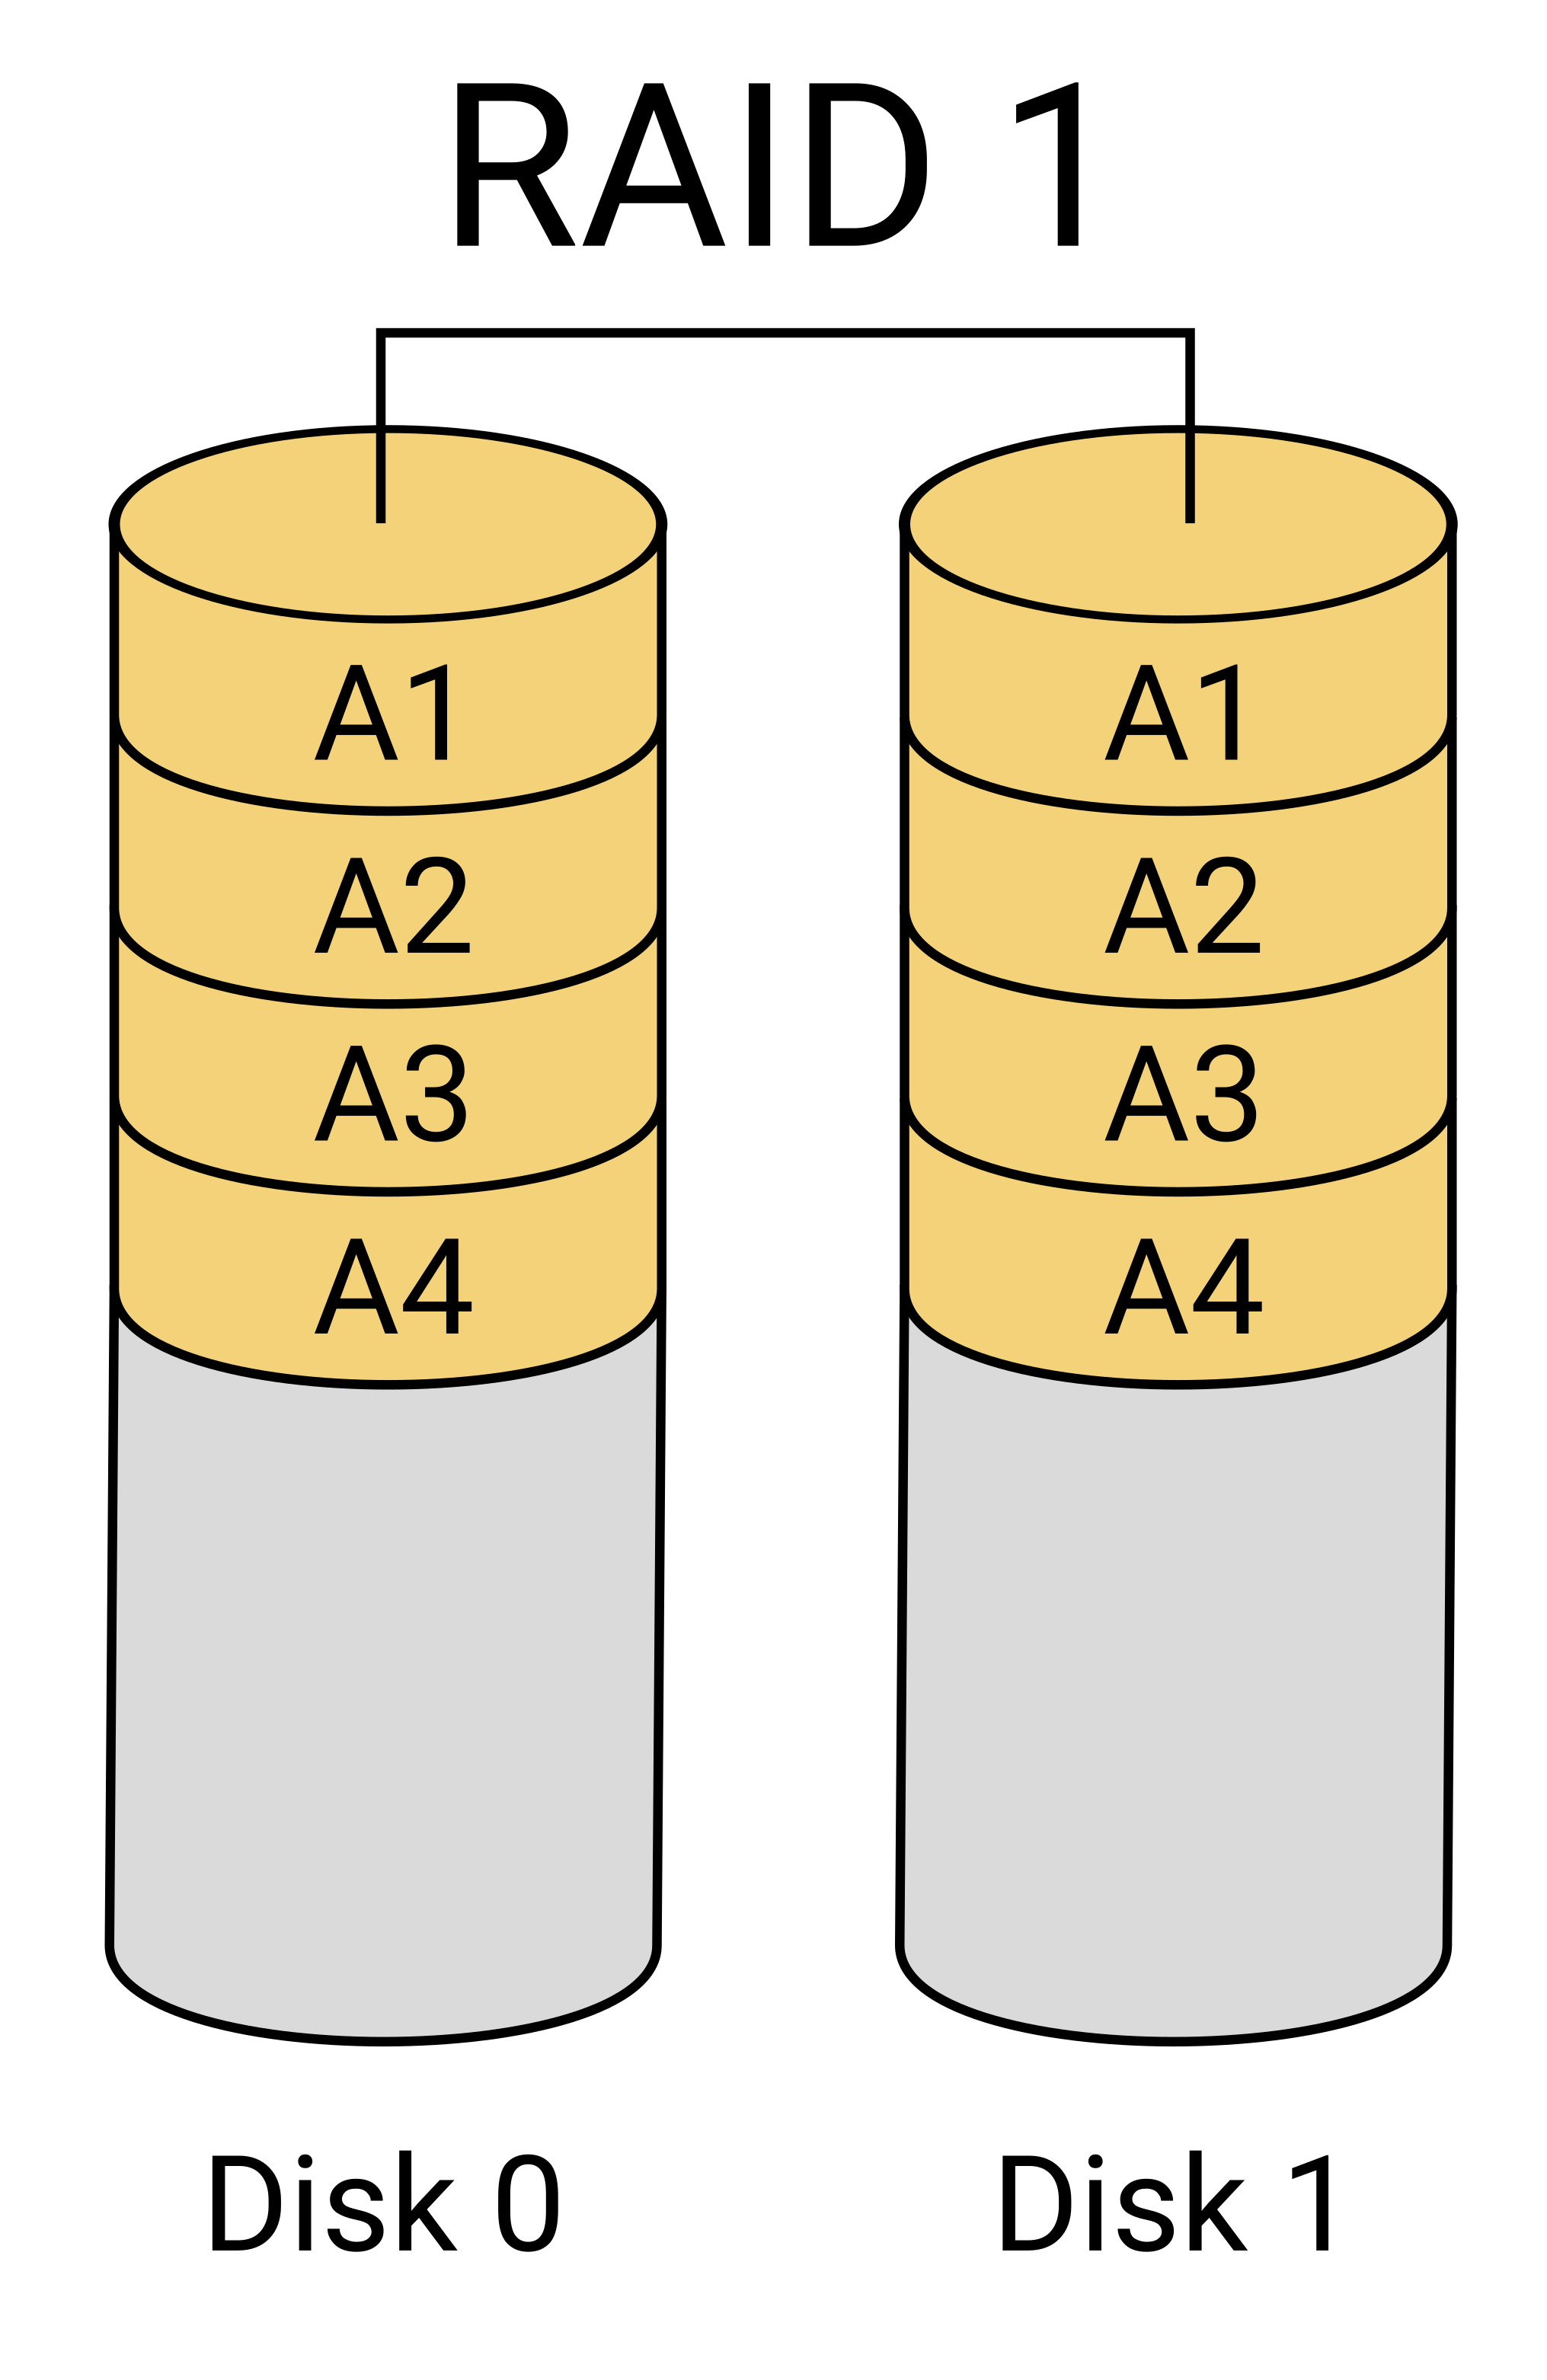
\includegraphics[keepaspectratio, height=52mm]{figures/raid1.pdf}
	\end{subfigure}
	\hspace{0.05\textwidth}
	\begin{subfigure}{0.6\textwidth}
		\centering
		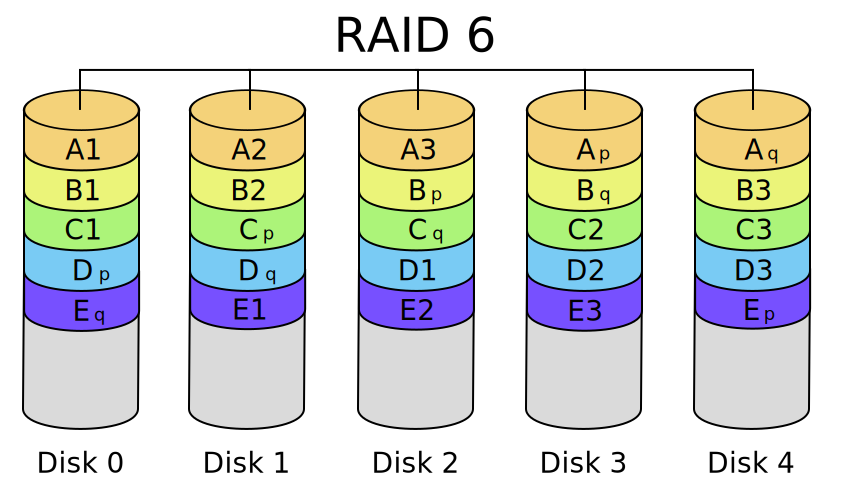
\includegraphics[keepaspectratio, height=52mm]{figures/raid6.pdf}
	\end{subfigure}
	\caption{RAID 1 és RAID 6 megoldások felépítése \cite{WikiRaidLevels}}
	\label{fig:raid}
\end{figure}


\section{Logikai kötetkezelés}
\label{sect:lvm}
Mind a fizikai, mind a virtuális gépek esetén szükség lehet háttértárakra az adatok perzisztens tárolása érdekében. Hagyományos particionálási megoldásokkal hamar nehezen kezelhetővé válhatnak a különböző csatolási pontok és a virtuális gépek számára kiosztott kötetek. Az ilyen problémák elkerülésére jött létre a logikai kötetkezelés, mely a tárhely-virtualizáció egy formája. A logikai kötetkezelésnek több implementációja létezik. % TODO: cite wikipedia: https://en.wikipedia.org/wiki/Logical_volume_management
Ezek közül jelenleg a Linux kernelben elérhető \gls{lvm}-et fogom részletesen ismertetni.

A Linux logikai kötetkezelője három lényegi rétegből áll: a fizikai kötetből (physical volume, PV), a kötetcsoportból (volume group, VG) és a logikai kötetekből (logical volume, LV). Ezt a felépítést \aref{fig:lvm} ábra szemlélteti egy egyszerű \gls{lvm}-konfiguráción keresztül.
Lehetőség van ennél összetettebb kötetkiosztás létrehozására is, például egy kötetcsoport több fizikai kötetből is állhat, amik akár külön háttértáron is lehetnek, sőt, RAID-csoportot is megadhatunk egy \gls{lvm}-partíció alapjául. Ezen megoldások használata azonban sok hátránnyal járhat (pl. diszkhiba esetén nehezebb visszaállítani a partíciót), ezért ennek használata alapvetően nem ajánlott~\cite{RHLVM}.

Az \gls{lvm} tehát úgy épül fel, hogy egy vagy több háttértáron létrehozunk hagyományos fizikai partíciókat, melyek az \gls{lvm} \acrshort{pv}-k alapjául fognak szolgálni. Ezt követően létrehozzuk a kötetcsoportokat az általuk használandó \acrshort{lvm} fizikai kötetek megadásával. Az így létrejött csoportban már tudunk létrehozni logikai köteteket, amíg van szabad hely a \acrshort{vg}-ben.

Láthatjuk, hogy az \acrshort{lvm}-kötetek használata kezdetben több feladattal jár, mint a hagyományos partíciók esetében, azonban hosszabb távon számos előnnyel jár. Talán a logikai kötetkezelés legnagyobb előnye, hogy szabadon allokálhatunk tárterületet a létrehozott köteteknek: ha azt tapasztaljuk, hogy az egyik köteten kevés a szabad hely, akkor fájlrendszertől függően elég lehet akár egy parancs kiadása is ennek kiterjesztéséhez. Lényeges, hogy a hagyományos partíciók használatával ellentétben a logikai kötetkezelés használatakor figyelmen kívül hagyhatjuk a partíciók elhelyezkedésének sorrendjét, így nem szükséges figyelembe vennünk, hogy az adott partíció előtt vagy után van-e szabad tárterület. A megnövelt kötet helyes fizikai háttértárra képzéséről a logikai kötetkezelő fog gondoskodni számunkra. Fontos megjegyezni, hogy a kötetbővítés online is elvégezhető, azaz nem szükséges a kötetet lecsatolni a gépről az átméretezéshez. Ez különösen fontos lehet például a root~(/) partíció növelése során, hiszen ezt csak a számítógép leállítása mellett tudjuk biztonságosan lecsatolni. Előállhat olyan helyzet is, hogy egy másik (nem root) partíciót kell online átméreteznünk, például ha azt tapasztaljuk, hogy egy adatbázisszerveren hirtelen nagy mértékben nőtt a tárolt adat mérete. Ilyenkor nincs lehetőség a szerver leállítására, hiszen ez esetben az alkalmazások nem tudnák használni az adatbázist a leállás idejére. Az ehhez hasonló helyzetekre is jó megoldást nyújt a logikai kötetkezelő egy megfelelő, online átméretezést támogató fájlrendszer (pl. XFS, Btrfs) használata mellett. Érdemes megjegyezni, hogy bár az \acrshort{lvm} és például a Btrfs-fájlrendszer nyújt támogatást a növelésen kívül a fájlrendszer méretének csökkentésére is, ez a művelet általában nem biztonságos, és adatvesztéshez vezethet. Emiatt érdemes eleinte csak kisebb tárterületet adni a köteteinknek, hiszen kiterjeszteni sokkal egyszerűbb őket, mint csökkenteni a méretüket. Ennek megkönnyítésére is ad lehetőséget az \acrshort{lvm}, megadhatjuk, hogy egy kötet egy bizonyos arányú tárhelyhasználat után automatikusan bővüljön, így elkerülve annak betelését.

Az \acrshort{lvm} hasznos funkciói közé tartozik még a kötetpillanatképek (volume snapshots) készítésének lehetősége. Ez azt jelenti, hogy a kötetkezelő képes az adott kötet adott pillanatbeli helyzetének rögzítésére, és erre a verzióra szükség szerint visszaállhatunk (rollback). Ez hasznos lehet például nagyobb konfigurációs változások eszközölése esetén, gyorsan változó adatokkal dolgozó rendszerek (pl. adatbázisszerver) biztonsági mentéseinek készítése során, illetve rendszerfrissítések előtt.\footnote{Egyes eszközök és operációs rendszerek (pl. openSUSE-verziók a snapper-rel (\url{https://doc.opensuse.org/documentation/leap/reference/html/book-reference/cha-snapper.html}) automatikusan készítenek snapshotot a frissítések telepítése előtt, így hiba esetén visszaállhatunk a frissítés előtti verzióra.}



\begin{figure}[!ht]
	\centering
	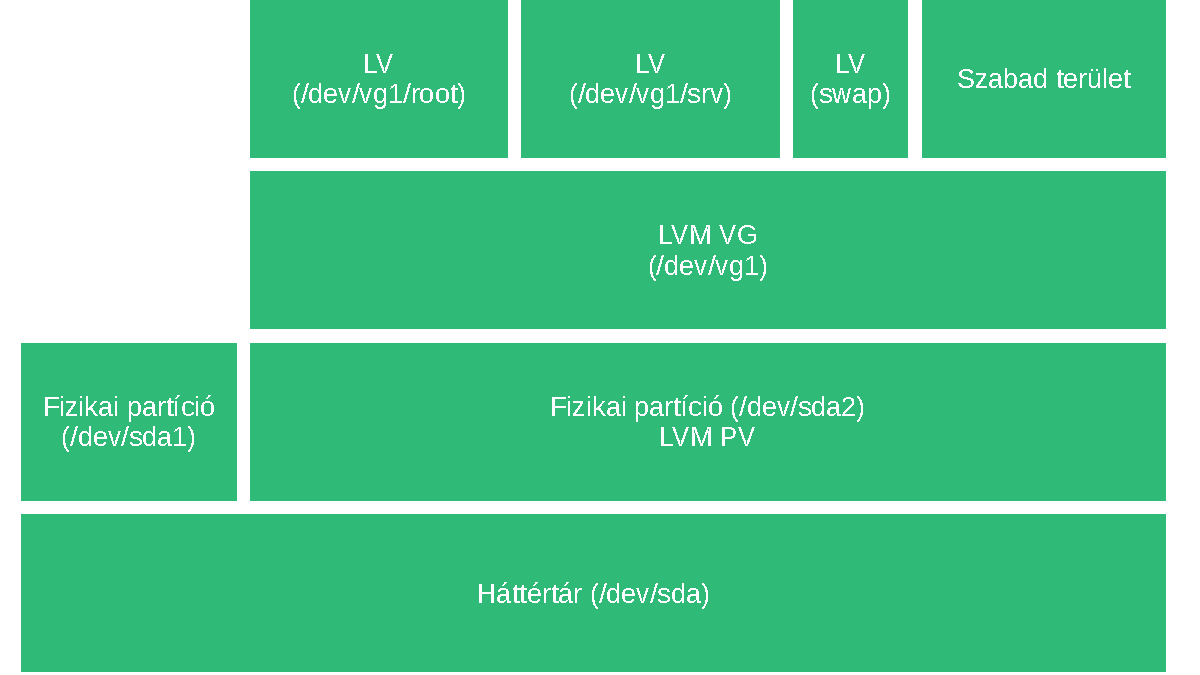
\includegraphics[width=14cm]{figures/lvm.pdf}
	\caption{Egyszerű \acrshort{lvm}-kötetkezelési hierarchia.}
	\label{fig:lvm}
\end{figure}

\section{OS-lehetőségek} \label{sect:os}
Egy nagyvállalati informatikai infrastruktúrában nagy szerepe van a választott operációs rendszernek is, ugyanis nem mindegy, hogy a több száz számítógépből álló rendszerünket mennyire hatékonyan tudjuk karban tartani, egy kritikus biztonsági frissítést milyen hamar tudunk telepíteni az érintett eszközökre, és probléma vagy különleges igény esetén milyen támogatásra számíthatunk a szoftvereinket illetően.
Ezeket a szempontokat figyelembe véve manapság elsősorban a Debian, Ubuntu, Red Hat Enterprise Linux és SUSE Linux Enterprise diszribúciók közül választanak a vállalatok.

A Debian stabilitása miatt népszerű választás elsősorban kisebb (néhány tíz gépből álló) infrastruktúrák esetében, viszont a stabilitás az elérhető csomagok verzióinak rovására megy, általában a legújabbnál néhány verzióval régebbi csomagokat szállítanak a disztribúcióval. A Debian előnye, hogy teljesen ingyenesen elérhető, és bár nincs hozzá hivatalos támogatás, harmadik féltől vásárolhatunk ilyen szolgáltatást.

Az Ubuntu egy Debian-alapú operációs rendszer, melyet a Canonical Ltd. fejleszt, és vállalati támogatást is nyújt az OS-hez amellett, hogy az alapverzió ingyenesen érhető el. Előnye, hogy mivel mind szerver, mind pedig asztali környezetben elterjedt rendszer, számtalan projekt és gyártó adja ki a szoftvereit Ubuntu rendszerekre.

A Red Hat és a SUSE Linux-verziók már inkább egy magasabb kategóriát céloznak meg: fő célközönségük a több száz, illetve több ezer gépes környezetet üzemeltető vállalatok, és a fent említett két disztribúciónál alapesetben (a legkisebb támogatási csomagban) is szélesebb körű támogatást biztosítanak az operációs rendszerekhez. Kiemelendő, hogy ez a két disztribúció egyedülálló a biztonság területén: számos biztonsági tesztnek vetették alá őket különböző szervezetek (köztük például kormányzatok és IT-biztonságra specializálódott cégek is), melyeket követően a kereskedelmi forgalomban lévő Linux-disztribúciók közül a legmagasabb minősítéseket és tanúsítványokat kapták meg ezek a rendszerek~\cite{RhSec}~\cite{SlesSec}.

Lényeges különbség még, hogy az utóbbi két operációs rendszer \acrshort{rpm}-alapú csomagkezelőt használ, mely a Debian és Ubuntu által használt DEB formátumhoz képest több lehetőséget biztosít például javítások (patchek) telepítésére. Emellett ez a formátum általában jobb támogatottságot élvez vállalati szoftverek esetében, ezért ezekben a felhasználási körökben az \acrshort{rpm}-csomagokat használnak a DEB-csomagokkal szemben.


\section{Infrastruktúramenedzsment}
Komplex infrastruktúrák esetén egyre nehezebbé válik a szerverek konfigurációjainak karbantartása, a frissítések kezelése. Manapság már széles körben elterjedtek az infrastruktúramenedzsment-megoldások, melyek lehetőséget biztosítanak ezen problémák kiküszöbölésére. Alkalmazásukkal hatékonyabbá tehető a számítógépek szoftveres karbantartása, könnyen egységesíthetőek a konfigurációs állományok, és így egyszerűbben kezelhetővé válnak az azonos szerepű számítógépek, rendszercsoportok.

\subsection{Ansible és Salt}
Dolgozatomhoz az Ansible-t és az Uyuni alapjául szolgáló Salt-ot vizsgáltam meg közelebbről. Mindkét megoldás elterjedtnek tekinthető, azonban a felépítésük nagyban különbözik.

Az Ansible sikere az egyszerűségében rejlik: az Ansible szerveren, az úgynevezett \textit{Control Node}-on kívül nincs szükség további komponensek telepítésére az alapvető funkciók használatához. Az Ansible nem használ dedikált kliensszoftvereket, ezért \textit{agentless}-nek nevezik, működése a push modellen alapul. A feladatok végrehajtását, konfigurációs fájlok elhelyezését úgynevezett Playbook-okkal adhatjuk meg, melyek YAML-ben írt leírófájlok. Egy-egy ilyen fájl több, egymástól független, tetszőleges komplexitású feladatot definiálhat. A \textit{Control Node} ezeket \acrshort{ssh}-n keresztül hajtja végre, ehhez a kliensek \acrshort{ssh}-kulcsát kell megadnunk. A megoldás előnye, hogy így az autentikáció és a kommunikáció titkosságának fenntartása is jelentősen egyszerűsödik, hiszen egy már jól bevált, biztonságos komponensen alapul~\cite{RedHatAnsibleVsSalt}.

Az Ansible-lel szemben a Saltot a kezelt rendszerekre is szükséges telepíteni. A Salt felépítése két kulcsfontosságú komponensre osztható: a Salt Masterre és a Salt Minionokra (emiatt \textit{agent-based} architektúrának nevezik). Minionoknak a kliensekre telepített komponenst nevezzük, mely a későbbiekben az úgynevezett Salt State-ekben meghatározott feladatok végrehajtásáért lesz felelős, melyeket a Master delegál ki a kliensek számára. A feladatleírók, a State-ek a Salt esetében is YAML-alapúak. A Salt architektúrájában a kezdeti kapcsolatfelvételt a minion indítja a publikus RSA-kulcsának elküldésével, ezt manuálisan kell ellenőrizni és elfogadni a Masteren. Ha a kulcs elfogadásra kerül, a szerver is elküldi a saját publikus kulcsát a Minionnak~\cite{SaltSecurity}. Ezt követően a Salt Master már képes a bevont Minionnak végrehajtandó feladatokat küldeni, valamint a Minion állapotát lekérdezni~\cite{RedHatAnsibleVsSalt}.

\section{Monitoring}
